\begin{sidewaysfigure}
    \centering
   % \footnotesize
    \setlength{\tabcolsep}{2pt}
    % First Row (4 columns)
    \begin{subfigure}[b]{0.23\textwidth}
        \centering
        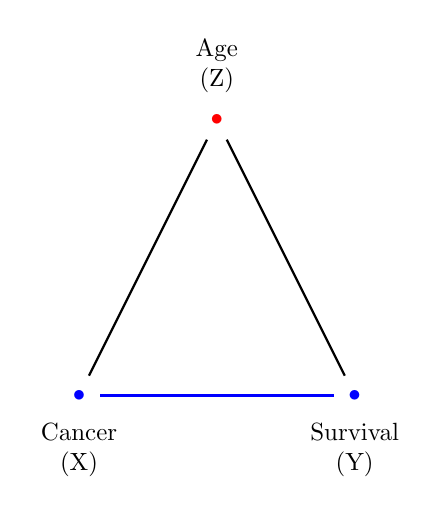
\begin{tikzpicture}[thick,scale=0.35, shorten >=2pt, shorten <=2pt, every node/.style={scale=0.9}]
            \node [red, label=above:{\begin{tabular}{c}Age\\(Z)\end{tabular}}] (a) at (5,10) {$\bullet$};
            \node [blue, label=below:{\begin{tabular}{c}Cancer\\(X)\end{tabular}}] (s) at (0,0) {$\bullet$};
            \node [blue, label=below:{\begin{tabular}{c}Survival\\(Y)\end{tabular}}] (x) at (10,0) {$\bullet$};
            \path (a) edge (s);
            \path[blue] (s) edge (x);
            \path (a) edge (x);
        \end{tikzpicture}
        \caption{Plain Vanilla Fork}
    \end{subfigure}
    \hfill
    \begin{subfigure}[b]{0.23\textwidth}
        \centering
        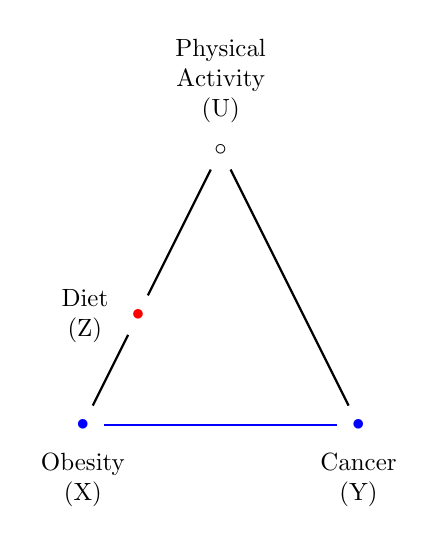
\begin{tikzpicture}[thick,scale=0.35, shorten >=2pt, shorten <=2pt, every node/.style={scale=0.9}]
            \node [label=above:{\begin{tabular}{c}Physical\\Activity\\(U)\end{tabular}}] (PA) at (5,10) {$\circ$};
            \node [red, label=left:{\begin{tabular}{c}Diet\\(Z)\end{tabular}}] (Diet) at (2,4) {$\bullet$};
            \node [blue, label=below:{\begin{tabular}{c}Obesity\\(X)\end{tabular}}] (Obesity) at (0,0) {$\bullet$};
            \node [blue, label=below:{\begin{tabular}{c}Cancer\\(Y)\end{tabular}}] (Cancer) at (10,0) {$\bullet$};
            \path (PA) edge (Diet);
            \path (Diet) edge (Obesity);
            \path[blue] (Obesity) edge (Cancer);
            \path (PA) edge (Cancer);
        \end{tikzpicture}
        \caption{Piping Fork on Causes}
    \end{subfigure}
    \hfill
    \begin{subfigure}[b]{0.23\textwidth}
        \centering
        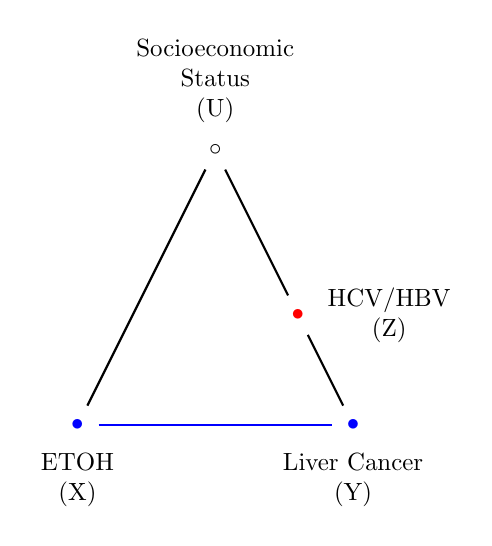
\begin{tikzpicture}[thick,scale=0.35, shorten >=2pt, shorten <=2pt, every node/.style={scale=0.9}]
            \node [label=above:{\begin{tabular}{c}Socioeconomic\\Status\\(U)\end{tabular}}] (SE) at (5,10) {$\circ$};
            \node [red, label=right:{\begin{tabular}{c}HCV/HBV\\(Z)\end{tabular}}] (HCV) at (8,4) {$\bullet$};
            \node [blue, label=below:{\begin{tabular}{c}ETOH\\(X)\end{tabular}}] (ETOH) at (0,0) {$\bullet$};
            \node [blue, label=below:{\begin{tabular}{c}Liver Cancer\\(Y)\end{tabular}}] (LiverCancer) at (10,0) {$\bullet$};
            \path (SE) edge (ETOH);
            \path[blue] (ETOH) edge (LiverCancer);
            \path (HCV) edge (LiverCancer);
            \path (SE) edge (HCV);
        \end{tikzpicture}
        \caption{Piping Fork on Effect}
    \end{subfigure}
    \hfill
    \begin{subfigure}[b]{0.23\textwidth}
        \centering
        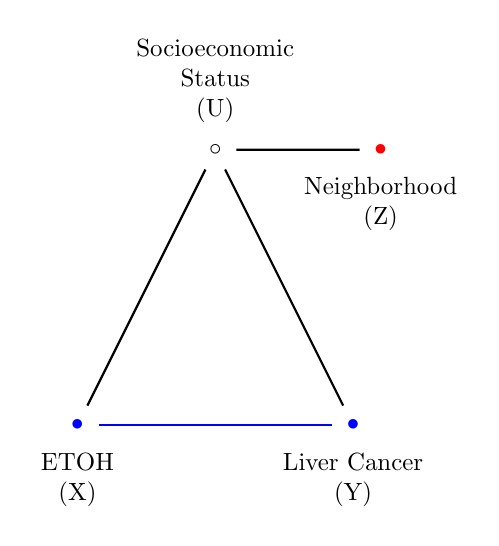
\begin{tikzpicture}[thick,scale=0.35, shorten >=2pt, shorten <=2pt, every node/.style={scale=0.9}]
            \node [label=above:{\begin{tabular}{c}Socioeconomic\\Status\\(U)\end{tabular}}] (SE) at (5,10) {$\circ$};
            \node [red, label=below:{\begin{tabular}{c}Neighborhood\\(Z)\end{tabular}}] (nb) at (11,10) {$\bullet$};
            \node [blue, label=below:{\begin{tabular}{c}ETOH\\(X)\end{tabular}}] (ETOH) at (0,0) {$\bullet$};
            \node [blue, label=below:{\begin{tabular}{c}Liver Cancer\\(Y)\end{tabular}}] (LiverCancer) at (10,0) {$\bullet$};
            \path (SE) edge (ETOH);
            \path[blue] (ETOH) edge (LiverCancer);
            \path (SE) edge (LiverCancer);
            \path (SE) edge (nb);
        \end{tikzpicture}
        \caption{Descendant of the Fork}
    \end{subfigure}

    \par\vspace{1em}

    % Second Row (4 columns)
    \begin{subfigure}[b]{0.23\textwidth}
        \centering
        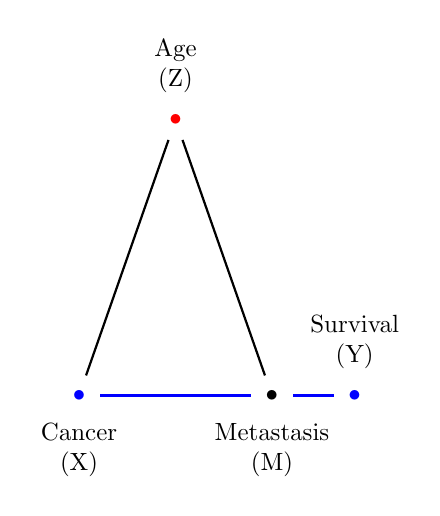
\begin{tikzpicture}[thick,scale=0.35, shorten >=2pt, shorten <=2pt, every node/.style={scale=0.9}]
            \node [red, label=above:{\begin{tabular}{c}Age\\(Z)\end{tabular}}] (Age) at (3.5,10) {$\bullet$};
            \node [blue, label=below:{\begin{tabular}{c}Cancer\\(X)\end{tabular}}] (CD) at (0,0) {$\bullet$};
            \node [label=below:{\begin{tabular}{c}Metastasis\\(M)\end{tabular}}] (Me) at (7,0) {$\bullet$};
            \node [blue, label=above:{\begin{tabular}{c}Survival\\(Y)\end{tabular}}] (Survival) at (10,0) {$\bullet$};
            \path (Age) edge (CD);
            \path (Age) edge (Me);
            \path[blue] (CD) edge (Me);
            \path[blue] (Me) edge (Survival);
        \end{tikzpicture}
        \caption{Mediated Fork}
    \end{subfigure}
    \hfill
    \begin{subfigure}[b]{0.23\textwidth}
        \centering
        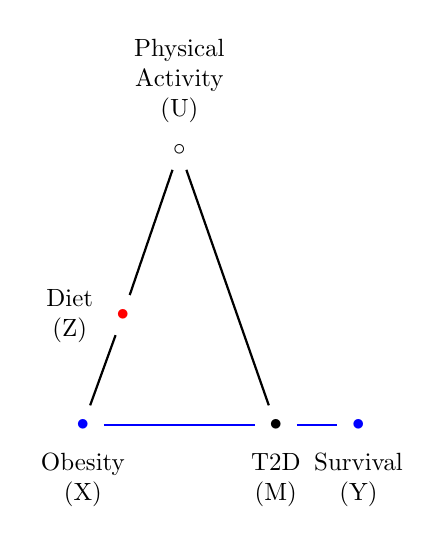
\begin{tikzpicture}[thick,scale=0.35, shorten >=2pt, shorten <=2pt, every node/.style={scale=0.9}]
            \node [label=above:{\begin{tabular}{c}Physical\\Activity\\(U)\end{tabular}}] (PA) at (3.5,10) {$\circ$};
            \node [red, label=left:{\begin{tabular}{c}Diet\\(Z)\end{tabular}}] (Diet) at (1.45,4) {$\bullet$};
            \node [blue, label=below:{\begin{tabular}{c}Obesity\\(X)\end{tabular}}] (Obesity) at (0,0) {$\bullet$};
            \node [label=below:{\begin{tabular}{c}T2D\\(M)\end{tabular}}] (T2D) at (7,0) {$\bullet$};
            \node [blue, label=below:{\begin{tabular}{c}Survival\\(Y)\end{tabular}}] (Survival) at (10,0) {$\bullet$};
            \path (PA) edge (Diet);
            \path (Diet) edge (Obesity);
            \path[blue] (Obesity) edge (T2D);
            \path (PA) edge (T2D);
            \path[blue] (T2D) edge (Survival);
        \end{tikzpicture}
        \caption{Mediated Fork on Cause}
    \end{subfigure}
    \hfill
    \begin{subfigure}[b]{0.23\textwidth}
        \centering
        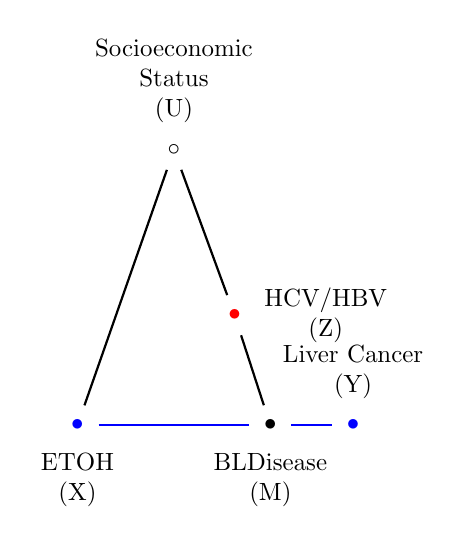
\begin{tikzpicture}[thick,scale=0.35, shorten >=2pt, shorten <=2pt, every node/.style={scale=0.9}]
            \node [label=above:{\begin{tabular}{c}Socioeconomic\\Status\\(U)\end{tabular}}] (SE) at (3.5,10) {$\circ$};
            \node [red, label=right:{\begin{tabular}{c}HCV/HBV\\(Z)\end{tabular}}] (HCV) at (5.7,4) {$\bullet$};
            \node [blue, label=below:{\begin{tabular}{c}ETOH\\(X)\end{tabular}}] (ETOH) at (0,0) {$\bullet$};
            \node [label=below:{\begin{tabular}{c}BLDisease\\(M)\end{tabular}}] (BLDisease) at (7,0) {$\bullet$};
            \node [blue, label=above:{\begin{tabular}{c}Liver Cancer\\(Y)\end{tabular}}] (LiverCancer) at (10,0) {$\bullet$};
            \path (SE) edge (ETOH);
            \path[blue] (ETOH) edge (BLDisease);
            \path (HCV) edge (BLDisease);
            \path (SE) edge (HCV);
            \path[blue] (BLDisease) edge (LiverCancer);
        \end{tikzpicture}
        \caption{Mediated Fork on Effect}
    \end{subfigure}
    \hfill
    \begin{subfigure}[b]{0.23\textwidth}
        \centering
        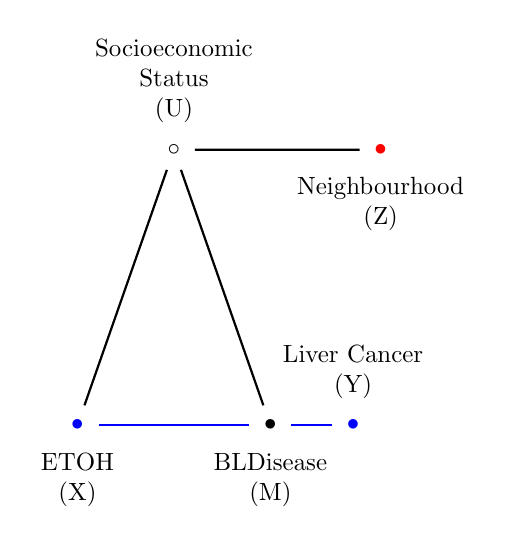
\begin{tikzpicture}[thick,scale=0.35, shorten >=2pt, shorten <=2pt, every node/.style={scale=0.9}]
            \node [label=above:{\begin{tabular}{c}Socioeconomic\\Status\\(U)\end{tabular}}] (SE) at (3.5,10) {$\circ$};
            \node [red, label=below:{\begin{tabular}{c}Neighbourhood\\(Z)\end{tabular}}] (NB) at (11,10) {$\bullet$};
            \node [blue, label=below:{\begin{tabular}{c}ETOH\\(X)\end{tabular}}] (ETOH) at (0,0) {$\bullet$};
            \node [label=below:{\begin{tabular}{c}BLDisease\\(M)\end{tabular}}] (BLDisease) at (7,0) {$\bullet$};
            \node [blue, label=above:{\begin{tabular}{c}Liver Cancer\\(Y)\end{tabular}}] (LiverCancer) at (10,0) {$\bullet$};
            \path (SE) edge (ETOH);
            \path[blue] (ETOH) edge (BLDisease);
            \path (SE) edge (BLDisease);
            \path (SE) edge (NB);
            \path[blue] (BLDisease) edge (LiverCancer);
        \end{tikzpicture}
        \caption{Descendant – Mediated Fork}
    \end{subfigure}

    \caption{\textbf{Fork Diagrams: Causal, Piping, and Mediated Structures}}
    \label{fig:fork_4x2}
\end{sidewaysfigure}
